
Для того, чтобы разобраться в том, как формируются экспериментальные
двухкристальные КДО, нам необходимо построить спектрально-угловое распределение
в соответствии со схемой эксперимента (рисунок \ref{ris:double_crystal_schem_lamtet_a}).

\begin{eqnarray} \label{eq:doudle_spectra_angle_map}
  P(\theta,\vartheta,\lambda) = g_{\lambda}(\lambda)g_{\vartheta}(\vartheta) P_M \left(\vartheta - \frac{\lambda - \lambda_1}{\lambda_1}\tan(\theta_B) \right) \cdot \nonumber \\
   P_S \left(\theta + \vartheta - \frac{\lambda - \lambda_1}{\lambda_1}\tan(\theta_B)\right)
 \end{eqnarray}

Выражение (\ref{eq:doudle_spectra_angle_map}) определяет спектрально угловое распределение после прохождения двух кристаллов с
коэффициентами отражения  $P_M$ (монохроматор) и $P_S$ (образец), причем последний принимает во внимание положение угла отстройки $\theta$ относительно
точного Брегга (рисунок \ref{ris:double_crystal_schem_lamtet_b}).

\begin{figure}[H]
  \centering
  \subfloat[Схема двухкристального эксперимента]{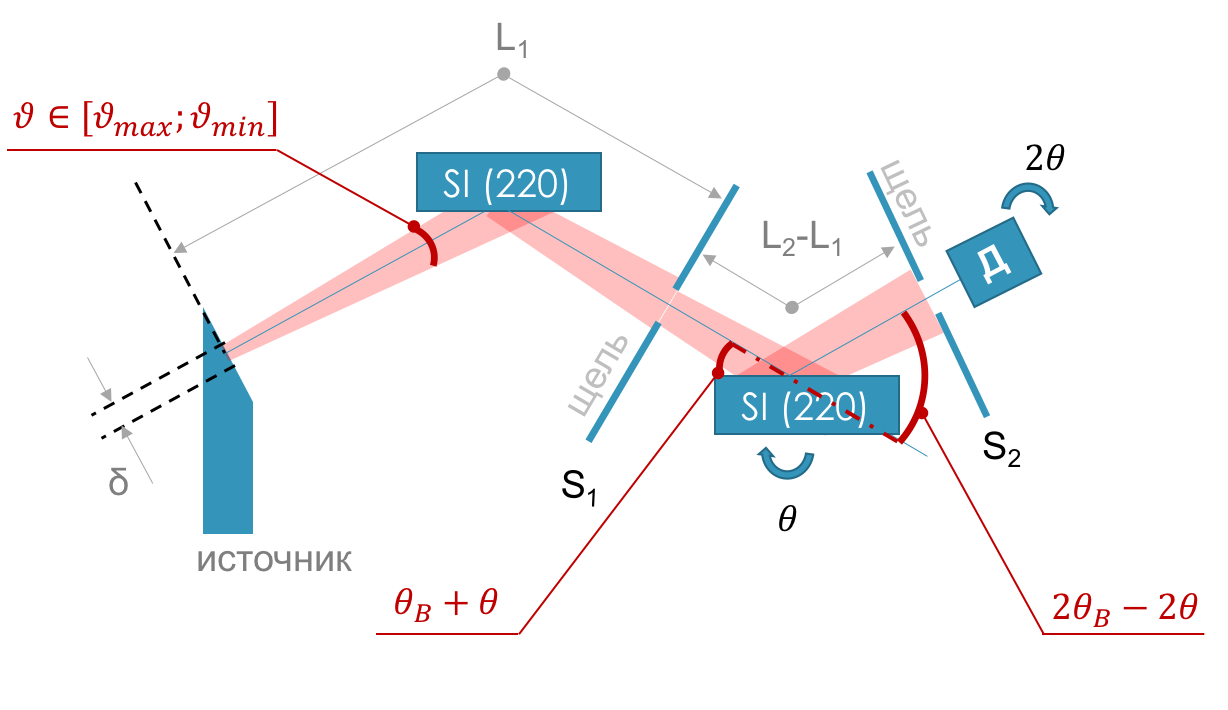
\includegraphics[width=0.5\textwidth]{images/double_crystal_schem.png}\label{ris:double_crystal_schem_lamtet_a}}
  \hfill
  \subfloat[Спектрально угловое распределение. Положение щелевых устройств обозначено синей и белой линиями вблизи $\vartheta = 0$ угл.сек. Кристалл-образец
  выведен из точного Брегговского положения на 300 угл. сек.
   ]{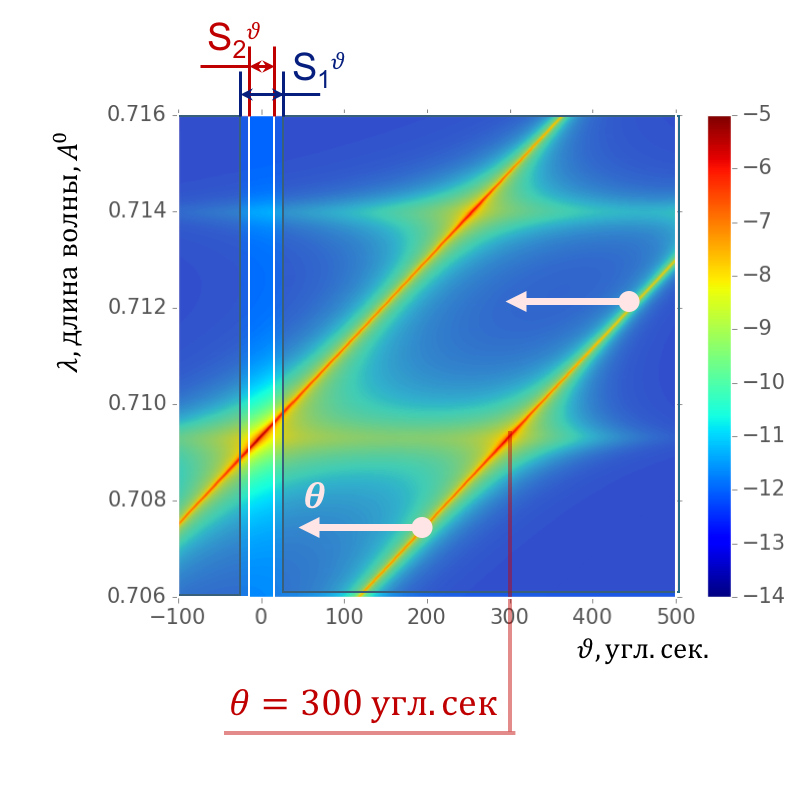
\includegraphics[width=0.45\textwidth]{images/double_crystal_schem_lamtet.png} \label{ris:double_crystal_schem_lamtet_b}}

  \caption{Схема и спектрально-угловое распределение после отражения расходящегося, полихромотического пучка. Несмотря на то, что в
  экспериментальной схеме детектор со щелью не стоят на месте, на карте обе щели $S_1$ и $S_2$ - неподвижны. }
  \label{ris:double_crystal_schem_lamtet}
\end{figure}

Выражение (\ref{eq:doudle_spectra_angle_map}) не учитывает особенности особенности влияния щелевых коллиматоров, о которым мы говорили в
(раздел \ref{sec:slits_section}), а так же тот факт, что детектор не разделят энергетическую составляющую пучка.


\begin{eqnarray} \label{eq:doudle_spectra_angle_map_on_detector}
  P_{double}(\theta) = \sum_{\lambda = -\infty}^{\infty}g_{\lambda}(\lambda)\cdot
  \sum_{\vartheta = \vartheta_{s1}}^{\vartheta_{s2}} g_{\vartheta}(\vartheta) g_{S}(\vartheta) \cdot \nonumber \\
   P_M \left(\vartheta - \frac{\lambda - \lambda_1}{\lambda_1}\tan(\theta_B) \right) \cdot \nonumber \\
   P_S \left(\theta + \vartheta - \frac{\lambda - \lambda_1}{\lambda_1}\tan(\theta_B)\right)
 \end{eqnarray}
 где пределы суммирования определяются как $\vartheta_{s2} = - \vartheta_{s1} = \frac{\delta+S_1}{2L_1}$.

 \begin{figure}[H]
   \centering
   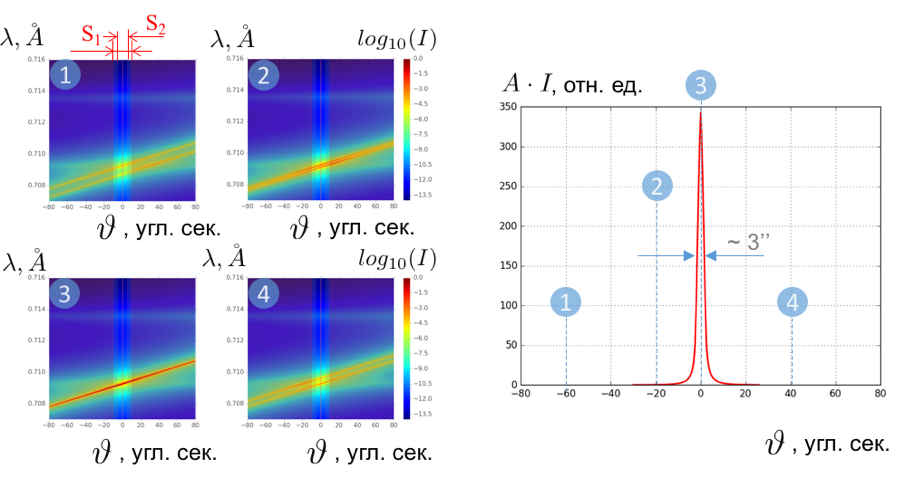
\includegraphics[width=1\textwidth]{images/double_crystal_form_kdo.png}
   \caption{Формирование двухкристальной кривой дифракционного отражения ($\theta - 2\theta$ - cканирование),
   $\theta_B^M = \theta_B^S = 10.6^o$  }
   \label{ris:double_crystal_form_kdo}
 \end{figure}

В том случае, если схема дисперсионная т.е. углол Брегга кристалла - образца отличен от угла Брега кристалла-монохроматора,
наблюдается уширения двухкристальных кривых (рисунок \ref{ris:double_crystal_form_kdo_dissp}).
 \begin{figure}[H]
   \centering
   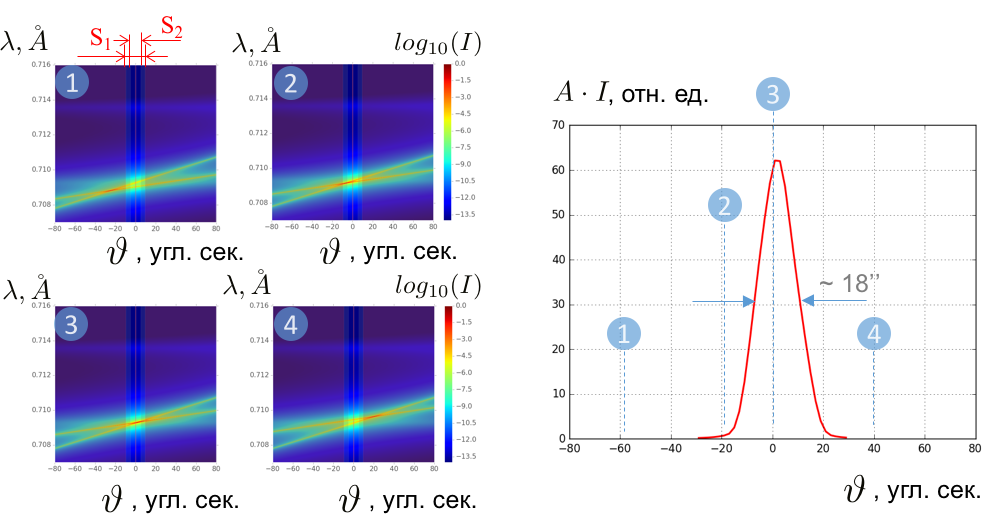
\includegraphics[width=1\textwidth]{images/double_crystal_form_kdo_dissp.png}
   \caption{Формирование двухкристальной кривой дифракционного отражения ($\theta - 2\theta$ - cканирование) в случае
   наличия дисперсии, $\theta_B^M = 10.6^o$, $\theta_B^S = 21.6^o$ }
   \label{ris:double_crystal_form_kdo_dissp}
 \end{figure}
